%%%%%%%%%%%%%%%%%%%%%%%%%%%%%%%%%%%%%%%%%%%%%%%%%%%%%%%%%%%%%%%%%%
%%%%%%%%%%%%%%%%%%%%%%%%%%%%%%%%%%%%%%%%%%%%%%%%%%%%%%%%%%%%%%%%%%
%Packages
\documentclass[10pt, a4paper]{article}
\usepackage[top=3cm, bottom=4cm, left=3.5cm, right=3.5cm]{geometry}
\usepackage{amsmath,amsthm,amsfonts,amssymb,amscd, fancyhdr, color, comment, graphicx, environ}
\usepackage{float}
\usepackage{mathrsfs}
\usepackage[math-style=ISO]{unicode-math}
\setmathfont{TeX Gyre Termes Math}
\usepackage{lastpage}
\usepackage[dvipsnames]{xcolor}
\usepackage[framemethod=TikZ]{mdframed}
\usepackage{enumerate}
\usepackage[shortlabels]{enumitem}
\usepackage{fancyhdr}
\usepackage{indentfirst}
\usepackage{listings}
\usepackage{sectsty}
\usepackage{thmtools}
\usepackage{shadethm}
\usepackage{hyperref}
\usepackage{setspace}
\hypersetup{
    colorlinks=true,
    linkcolor=blue,
    filecolor=magenta,      
    urlcolor=blue,
}
\usepackage[makeroom]{cancel}
\usepackage[utf8]{inputenc}
\usepackage[T1]{fontenc}
\usepackage{hyperref}
\hypersetup{colorlinks=true, linkcolor=blue, filecolor=magenta, urlcolor=cyan,}
\urlstyle{same}
\usepackage{amsmath}
\usepackage{amsfonts}
\usepackage{amssymb}
\usepackage[version=4]{mhchem}
\usepackage{stmaryrd}
\usepackage{graphicx}
\usepackage[export]{adjustbox}
\graphicspath{ {./images/} }
\usepackage{listings}
%%%%%%%%%%%%%%%%%%%%%%%%%%%%%%%%%%%%%%%%%%%%%%%%%%%%%%%%%%%%%%%%%%
%%%%%%%%%%%%%%%%%%%%%%%%%%%%%%%%%%%%%%%%%%%%%%%%%%%%%%%%%%%%%%%%%%
%Environment setup
\mdfsetup{skipabove=\topskip,skipbelow=\topskip}
\newrobustcmd\ExampleText{%
An \textit{inhomogeneous linear} differential equation has the form
\begin{align}
L[v ] = f,
\end{align}
where $L$ is a linear differential operator, $v$ is the dependent
variable, and $f$ is a given non−zero function of the independent
variables alone.
}
\mdfdefinestyle{theoremstyle}{%
linecolor=black,linewidth=1pt,%
frametitlerule=true,%
frametitlebackgroundcolor=gray!20,
innertopmargin=\topskip,
}
\mdtheorem[style=theoremstyle]{Problem}{Problem}
\newenvironment{Solution}{\textbf{Solution.}}

\definecolor{codegreen}{rgb}{0,0.6,0}
\definecolor{codegray}{rgb}{0.5,0.5,0.5}
\definecolor{codepurple}{rgb}{0.58,0,0.82}
\definecolor{backcolour}{rgb}{0.95,0.95,0.92}

\lstdefinestyle{mystyle}{
    backgroundcolor=\color{backcolour},   
    commentstyle=\color{codegreen},
    keywordstyle=\color{magenta},
    numberstyle=\tiny\color{codegray},
    stringstyle=\color{codepurple},
    basicstyle=\ttfamily\footnotesize,
    breakatwhitespace=false,         
    breaklines=true,                 
    captionpos=b,                    
    keepspaces=true,                 
    numbers=left,                    
    numbersep=5pt,                  
    showspaces=false,                
    showstringspaces=false,
    showtabs=false,                  
    tabsize=2
}

\lstset{style=mystyle}
%%%%%%%%%%%%%%%%%%%%%%%%%%%%%%%%%%%%%%%%%%%%%%%%%%%%%%%%%%%%%%%%%%
%%%%%%%%%%%%%%%%%%%%%%%%%%%%%%%%%%%%%%%%%%%%%%%%%%%%%%%%%%%%%%%%%%
%Fill in the appropriate information below
\newcommand{\norm}[1]{\left\lVert#1\right\rVert}     
\newcommand\course{CS5785}                            % <-- course name   
\newcommand\hwnumber{1}                                 % <-- homework number
\newcommand\Information{Arystan Tatishev, Maanas Peri}                        % <-- personal information
%%%%%%%%%%%%%%%%%%%%%%%%%%%%%%%%%%%%%%%%%%%%%%%%%%%%%%%%%%%%%%%%%%
%%%%%%%%%%%%%%%%%%%%%%%%%%%%%%%%%%%%%%%%%%%%%%%%%%%%%%%%%%%%%%%%%%
%Page setup
\pagestyle{fancy}
\headheight 35pt
\lhead{\today}
\rhead{
\includegraphics[width=2.5cm]{logo-ct.png}}
\lfoot{}
\pagenumbering{arabic}
\cfoot{\small\thepage}
\rfoot{}
\headsep 1.2em
\renewcommand{\baselinestretch}{1.25}
%%%%%%%%%%%%%%%%%%%%%%%%%%%%%%%%%%%%%%%%%%%%%%%%%%%%%%%%%%%%%%%%%%
%%%%%%%%%%%%%%%%%%%%%%%%%%%%%%%%%%%%%%%%%%%%%%%%%%%%%%%%%%%%%%%%%%
%Add new commands here
\renewcommand{\labelenumi}{\alph{enumi})}
\newcommand{\Z}{\mathbb Z}
\newcommand{\R}{\mathbb R}
\newcommand{\Q}{\mathbb Q}
\newcommand{\NN}{\mathbb N}
\newcommand{\PP}{\mathbb P}
\DeclareMathOperator{\Mod}{Mod} 
\renewcommand\lstlistingname{Algorithm}
\renewcommand\lstlistlistingname{Algorithms}
\def\lstlistingautorefname{Alg.}
\newtheorem*{theorem}{Theorem}
\newtheorem*{lemma}{Lemma}
\newtheorem{case}{Case}
\newcommand{\assign}{:=}
\newcommand{\infixiff}{\text{ iff }}
\newcommand{\nobracket}{}
\newcommand{\backassign}{=:}
\newcommand{\tmmathbf}[1]{\ensuremath{\boldsymbol{#1}}}
\newcommand{\tmop}[1]{\ensuremath{\operatorname{#1}}}
\newcommand{\tmtextbf}[1]{\text{{\bfseries{#1}}}}
\newcommand{\tmtextit}[1]{\text{{\itshape{#1}}}}

\newenvironment{itemizedot}{\begin{itemize} \renewcommand{\labelitemi}{$\bullet$}\renewcommand{\labelitemii}{$\bullet$}\renewcommand{\labelitemiii}{$\bullet$}\renewcommand{\labelitemiv}{$\bullet$}}{\end{itemize}}
\catcode`\<=\active \def<{
\fontencoding{T1}\selectfont\symbol{60}\fontencoding{\encodingdefault}}
\catcode`\>=\active \def>{
\fontencoding{T1}\selectfont\symbol{62}\fontencoding{\encodingdefault}}
\catcode`\<=\active \def<{
\fontencoding{T1}\selectfont\symbol{60}\fontencoding{\encodingdefault}}

%%%%%%%%%%%%%%%%%%%%%%%%%%%%%%%%%%%%%%%%%%%%%%%%%%%%%%%%%%%%%%%%%%
%%%%%%%%%%%%%%%%%%%%%%%%%%%%%%%%%%%%%%%%%%%%%%%%%%%%%%%%%%%%%%%%%%
%Begin now!



\begin{document}

\begin{titlepage}
    \begin{center}
        \vspace*{3cm}
            
        \Huge
        \textbf{Assignment}
            
        \vspace{1cm}
        \huge
        Homework\hwnumber
            
        \vspace{1.5cm}
        \Large
            
        \textbf{\Information}                      % <-- author
        
            
        \vfill
        
        A \course \ Homework Assignment
            
        \vspace{1cm}
            
        
\includegraphics[width=0.4\textwidth]{logo-ct.png}
        \\
        
        \Large
        
        \today
            
    \end{center}
\end{titlepage}

%%%%%%%%%%%%%%%%%%%%%%%%%%%%%%%%%%%%%%%%%%%%%%%%%%%%%%%%%%%%%%%%%%
%%%%%%%%%%%%%%%%%%%%%%%%%%%%%%%%%%%%%%%%%%%%%%%%%%%%%%%%%%%%%%%%%%
%Start the assignment now
%%%%%%%%%%%%%%%%%%%%%%%%%%%%%%%%%%%%%%%%%%%%%%%%%%%%%%%%%%%%%%%%%%
%New problem
\newpage
\section*{Coding Exercises}
\section*{Part I: The Housing Prices}
\setcounter{Problem}{1}
\begin{Problem}
Give 3 examples of continuous and categorical features in the dataset; choose one feature of each type and plot the histogram to illustrate the distribution.
\end{Problem}

\begin{Solution}

\begin{lstlisting}[language=Python]
    import pandas as pd
    import numpy as np 
    import matplotlib.pyplot as plt\end{lstlisting}
\begin{lstlisting}[language=Python]
    training_data = pd.read_csv("house-prices-advanced-regression-techniques/train.csv")
    testing_data = pd.read_csv("house-prices-advanced-regression-techniques/test.csv")
    training_data.head()\end{lstlisting}
\begin{lstlisting}[language=Python]
    continuous_features = training_data.select_dtypes(include=[np.number]) #used chatgpt to figure out how to select 
    categorical_features = training_data.select_dtypes(exclude=[np.number])
    continuous_features.head()
    categorical_features.head()\end{lstlisting}
    
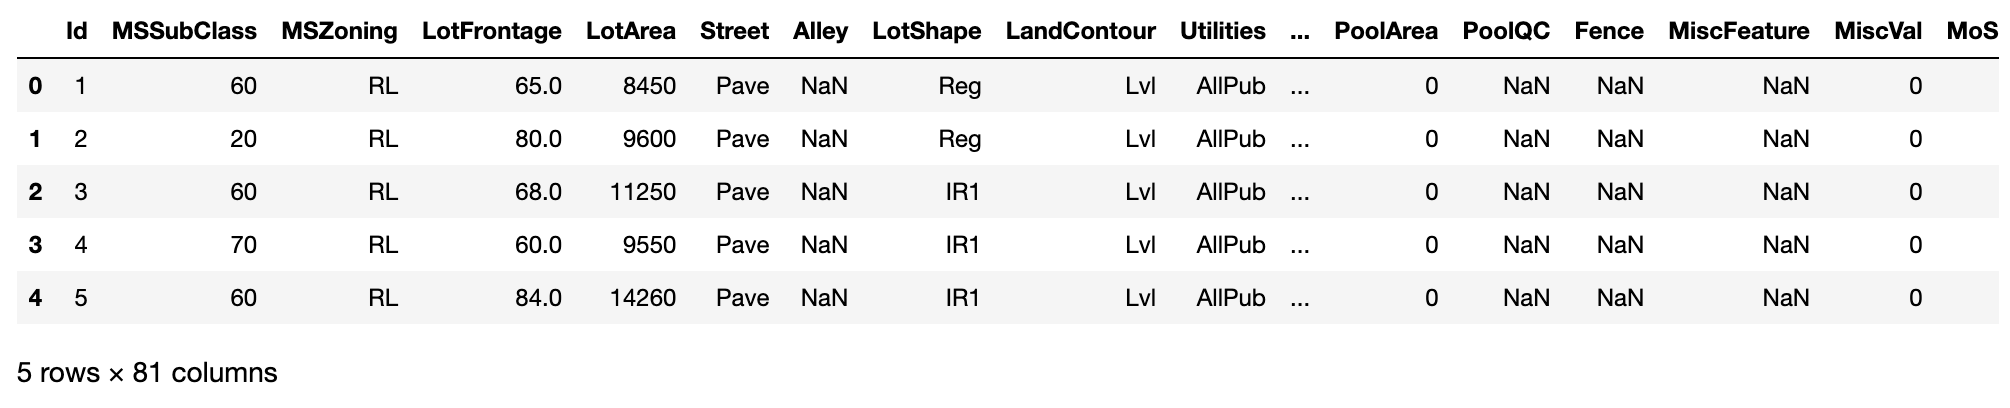
\includegraphics[max width=\textwidth, scale=1.0]{HW1/images/img1.png}
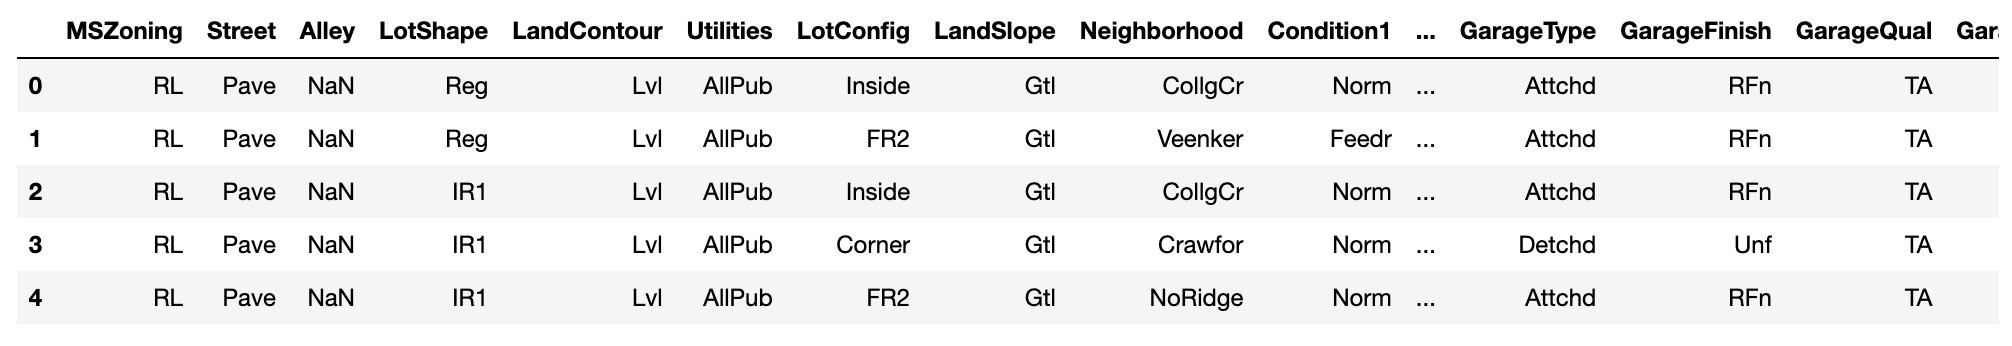
\includegraphics[max width=\textwidth, scale=1.0]{HW1/images/img2.png}

\begin{lstlisting}[language=Python]
    #selecting 3 variables - 2 continuous variables and 1 categorical variable
    lotArea = "LotArea"
    lotFrontage = "LotFrontage"
    lotConfig = "LotConfig"\end{lstlisting}

Here are the histograms of the 3 examples of continuous and categorical variables shown earlier.   

\begin{lstlisting}[language=Python]
    plt.figure(figsize=(10, 5))
    plt.hist(training_data[lotFrontage], bins=100, edgecolor='k')
    plt.title('Histogram of Continuous Feature ~ Lot Frontage')
    plt.xlabel('Value')
    plt.ylabel('Frequency')
    plt.show()\end{lstlisting}
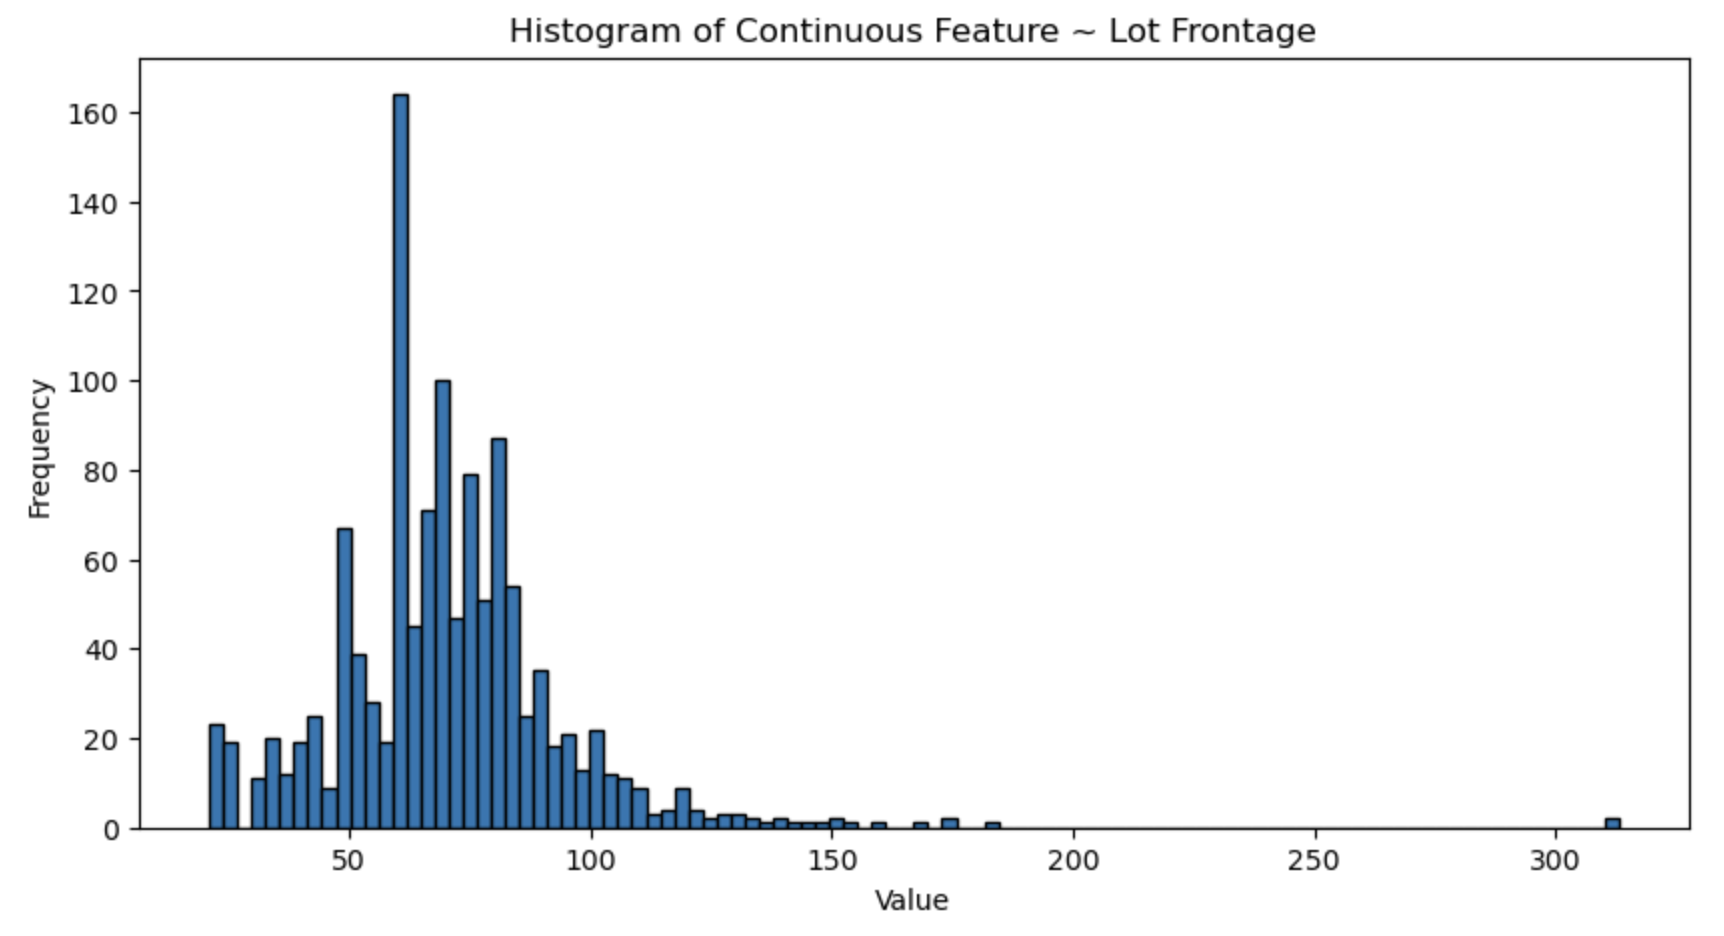
\includegraphics[max width=\textwidth, scale=1.0]{HW1/images/img3.png}

\begin{lstlisting}[language=Python]
    plt.figure(figsize=(10, 5))
    plt.hist(training_data[lotArea], bins=100, edgecolor='k')
    plt.title('Histogram of Continuous Feature ~ Lot Area')
    plt.xlabel('Value')
    plt.ylabel('Frequency')
    plt.show()\end{lstlisting}
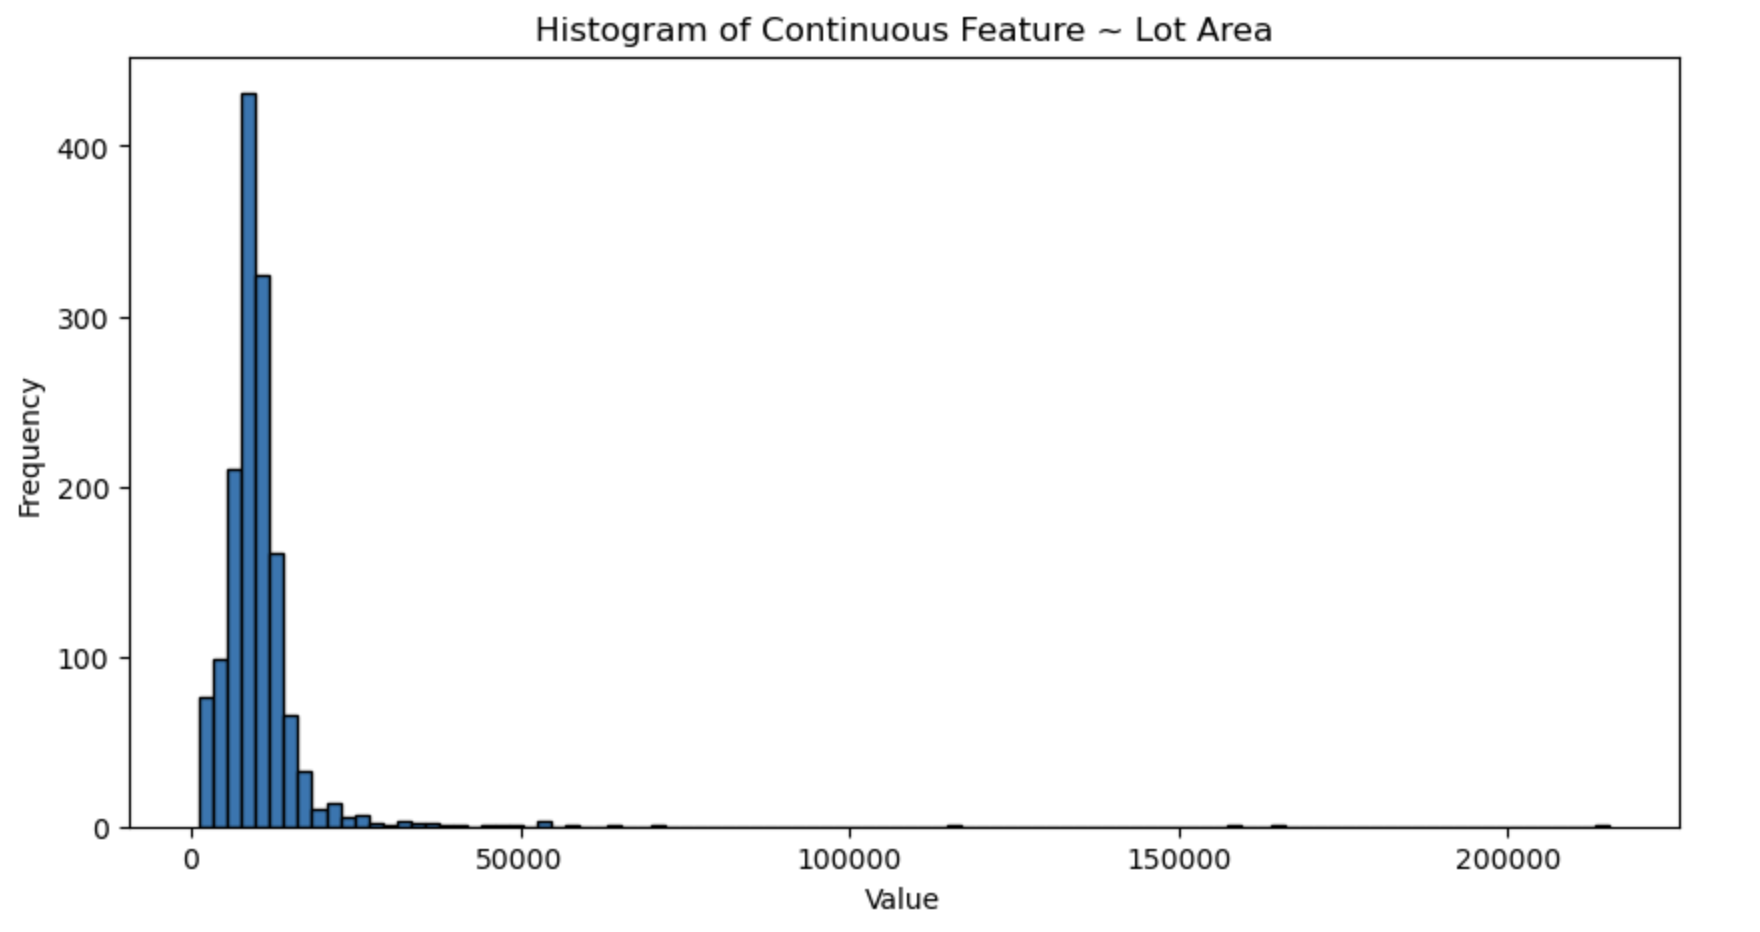
\includegraphics[max width=\textwidth, scale=1.0]{HW1/images/img4.png}

\begin{lstlisting}[language=Python]
    plt.figure(figsize=(10, 5))
    plt.hist(training_data[lotConfig], bins=100, edgecolor='k')
    plt.title('Histogram of Categorical Feature ~ LotConfig')
    plt.xlabel('Value')
    plt.ylabel('Frequency')
    plt.show()\end{lstlisting}
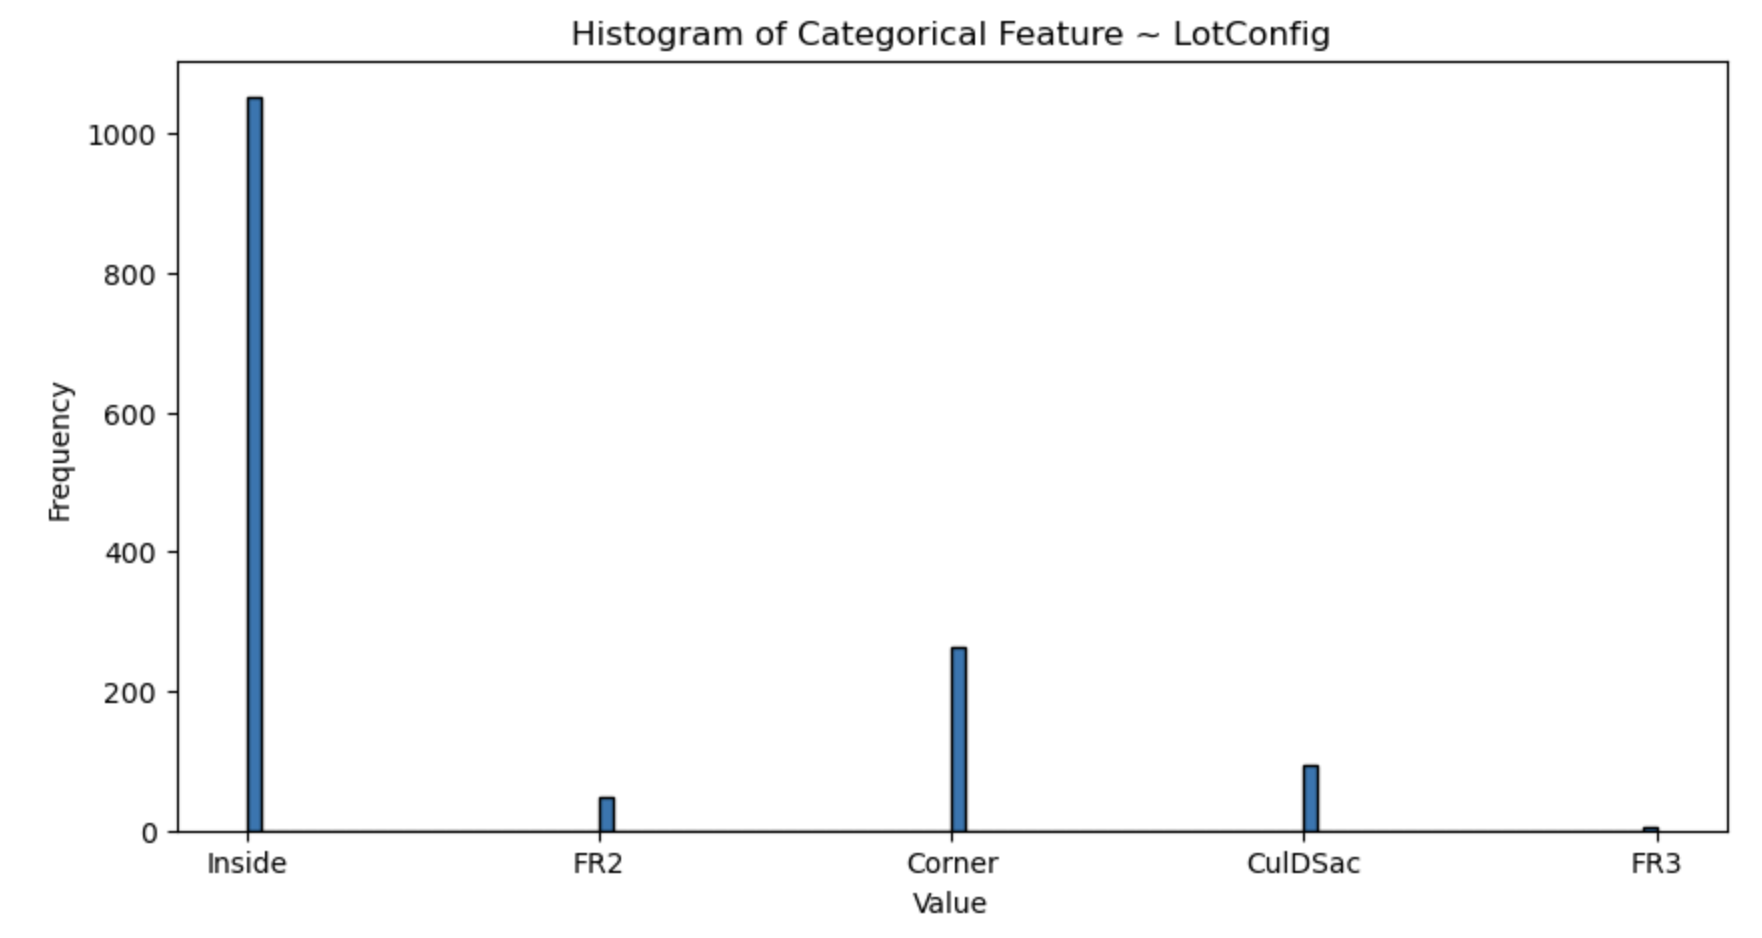
\includegraphics[max width=\textwidth, scale=1.0]{HW1/images/img5.png}


\end{Solution}

\begin{Problem}
Pre-process your data, explain your pre-processing steps, and the reasons why you need them. 
(Hint: data pre-processing steps can include but are not restricted to: dealing with missing values,
normalizing numerical values, dealing with categorical values etc.)
\end{Problem}

\begin{Solution}

First we are going to print out our training data information and see the count of the column variables that have non-null values. Our objective is to get the non-null count of all these columns up to a 1460 count.

\begin{enumerate}
    \item We need to first calculate if we even want to consider some columns, since they might be mostly made up of only a handful of non-null values. We can compute the percentage of missing values, and if consists of more than 33\% of the values, then we can eliminate the column completely, since we won't be able to extrapolate/learn much from it

    \item Next, of the columns that we want to process (and only have a few null values) we need to handle missing continuous and categorical data separately. For missing continuous values, we need to replace them with the mean of the columns as to not affect the distribution of the continuous variable and serve as a consistent representative of the feature. Next, we are going to encode our categorical features into a numerical format (0s and 1s) to make it compatible with our model. This transformation will allow our model to work with our categorical data effectively. 
\end{enumerate}

Incorporating these steps ensures that our model can derive meaningful patterns and make accurate predictions. 

\begin{lstlisting}[language=Python]
print(training_data.info())\end{lstlisting}

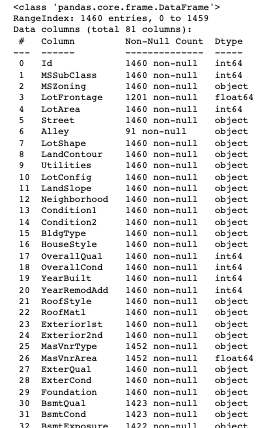
\includegraphics[max width=\textwidth, scale=1.0]{HW1/images/img6.png}
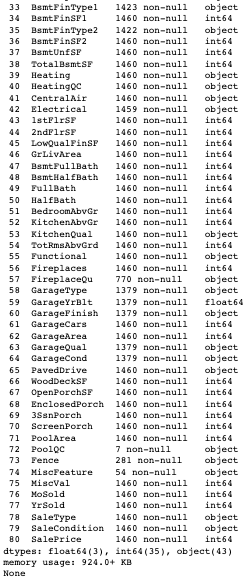
\includegraphics[max width=\textwidth, scale=1.0]{HW1/images/img7.png}

\begin{lstlisting}[language=Python]
processing_data = training_data
missing_percentage = (processing_data.isnull().sum() / len(training_data)) * 100
columns_to_remove = missing_percentage[missing_percentage > 33].index.tolist()
# print(columns_to_remove)
cleaned_data = processing_data.drop(columns=columns_to_remove)
# print(cleaned_data.info())

#replace the continuous variables from null values to mean() 
continuous_features = cleaned_data.select_dtypes(include=[np.number])
categorical_features = cleaned_data.select_dtypes(exclude=[np.number])
#replace the discrete variables from null values to 

#processing the continuous features first, by filling in all the null values with the mean of values, this way the distribution of this data won't get affected 
mean_values = continuous_features.mean()
continuous_features.fillna(mean_values, inplace=True)
# print(continuous_features.info()) #now we filled in the missing naan values with the mean value
\end{lstlisting}
    
\end{Solution}

\begin{Problem}
    One common method of pre-processing categorical features is to use a one-hot encoding (OHE).
    
Suppose that we start with a categorical feature $x_{j}$, taking three possible values: $x_{j} \in\{R, G, B\}$. A one-hot encoding of this feature replaces $x_{j}$ with three new features: $x_{j R}, x_{j G}, x_{j B}$. Each feature contains a binary value of 0 or 1 , depending on the value taken by $x_{j}$. For example, if $x_{j}=G$, then $x_{j G}=1$ and $x_{j R}=x_{j B}=0$.

Give some examples of features that you think should use a one-hot encoding and explain why. Convert at least one feature to a one-hot encoding (you can use your own implementation, or that in pandas or scikit-learn) and visualize the results by plotting feature histograms of the original feature and its new one-hot encoding.

\end{Problem}
The following list of categorical features that need encoding are below:
\begin{lstlisting}[language=Python]
['MSZoning', 'Street', 'LotShape', 'LandContour', 'Utilities', 'LotConfig', 'LandSlope', 'Neighborhood', 'Condition1', 'Condition2', 'BldgType', 'HouseStyle', 'RoofStyle', 'RoofMatl', 'Exterior1st', 'Exterior2nd', 'MasVnrType', 'ExterQual', 'ExterCond', 'Foundation', 'BsmtQual', 'BsmtCond', 'BsmtExposure', 'BsmtFinType1', 'BsmtFinType2', 'Heating', 'HeatingQC', 'CentralAir', 'Electrical', 'KitchenQual', 'Functional', 'GarageType', 'GarageFinish', 'GarageQual', 'GarageCond', 'PavedDrive', 'SaleType', 'SaleCondition']
\end{lstlisting}

We chose one-hot encoding for all of these features because all of them have discrete values that cannot have any arithmetic operations performed on them. If 'LotConfig'  = 'Inside', our model is going to have a hard time performing variant and loss operations on it (essentially having issues quantifying this 'Reg value'). That's why it's important to create new subcategories and use binary values to determine the proper 'LotConfig' attributes. 

For example, the original representation of the LotConfig is as we discussed above: 
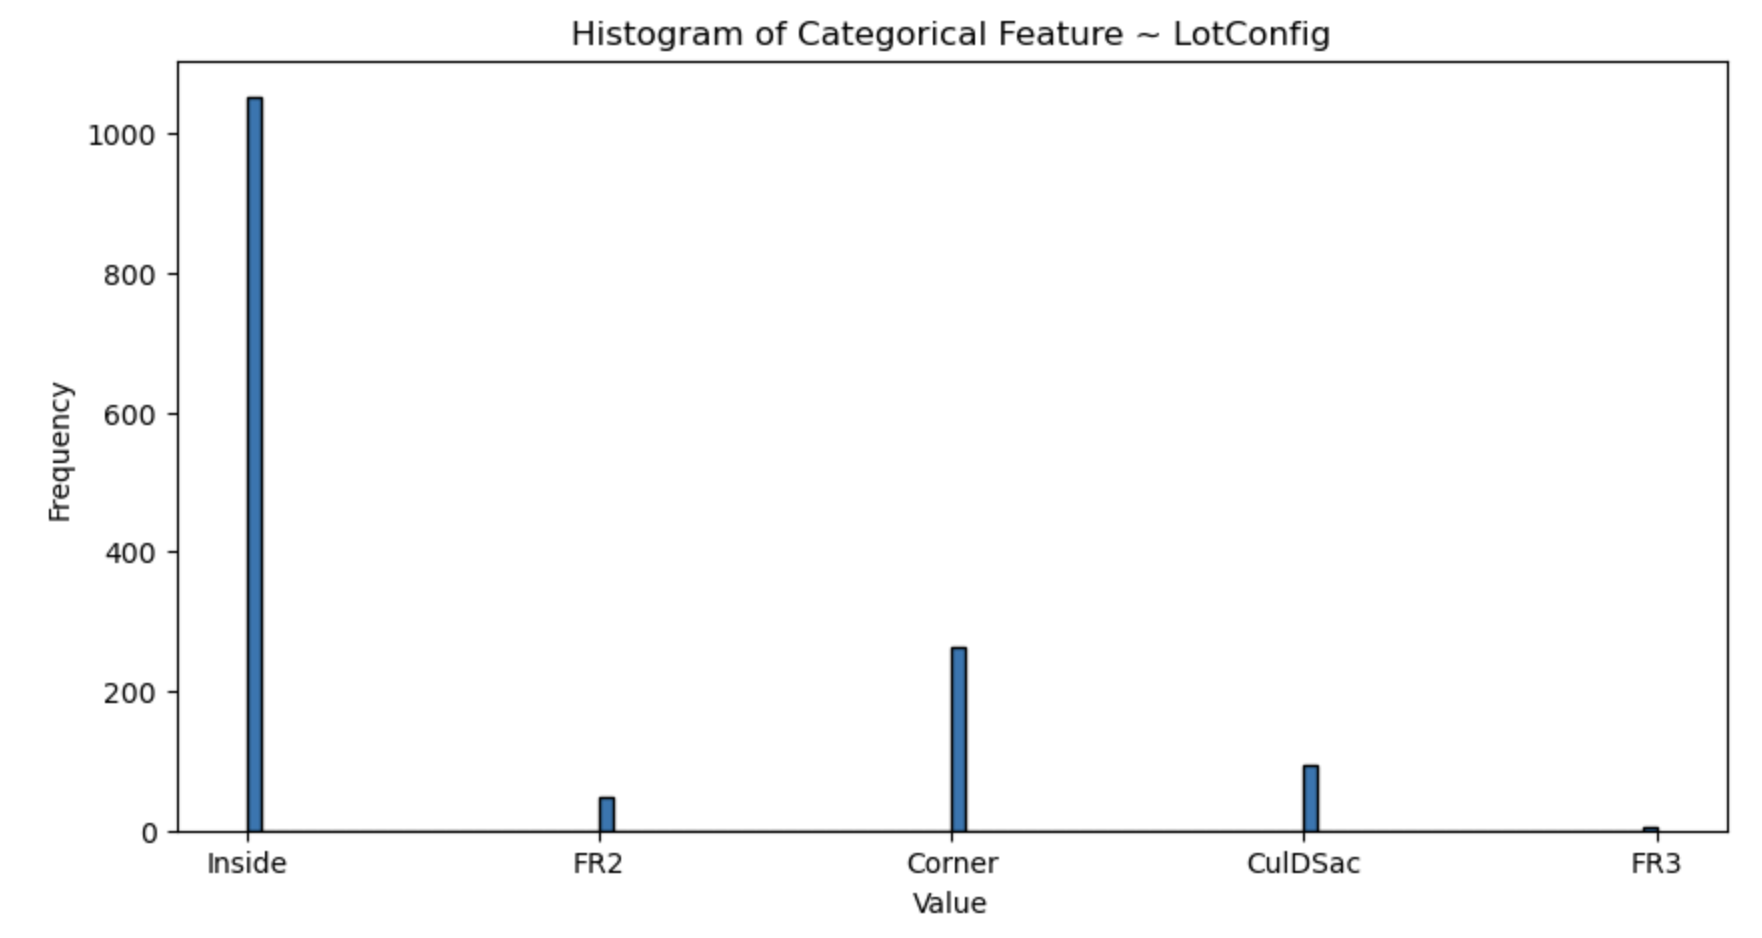
\includegraphics[max width=\textwidth, scale=1.0]{HW1/images/img5.png}

After performing a one-hot encoding program (below) on this specific categorical feature, we can understand how this histogram transformed, thereby reflecting the data. 

\begin{lstlisting}[language=Python]
newCategoricalData = pd.DataFrame()
newCategoricalData = pd.get_dummies(training_data[lotConfig])

for column in newCategoricalData.columns:
    plt.hist(newCategoricalData[column], bins=2, edgecolor='k')  # Assuming binary encoded (0s and 1s)
    plt.title(f'Histogram of Encoded Feature - {column}')
    plt.xlabel('Value')
    plt.ylabel('Frequency')
    plt.show()
\end{lstlisting}

This gives us the following graphs: 
\begin{figure*}[ht!]
    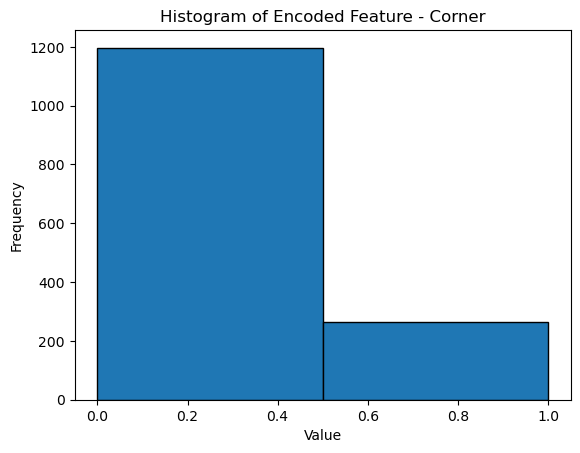
\includegraphics[width=.5\textwidth]{HW1/images/download.png}\hfill
    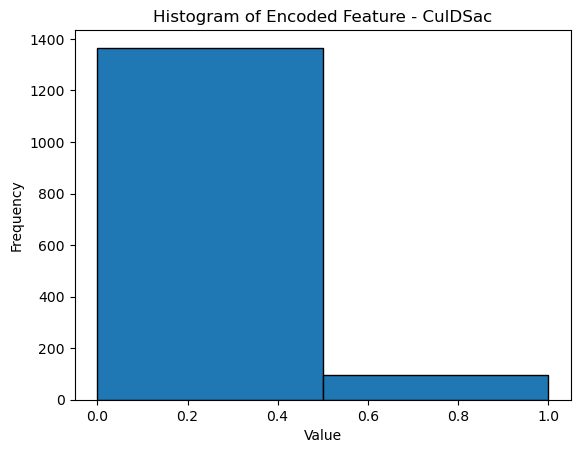
\includegraphics[width=.5\textwidth]{HW1/images/download2.png}\hfill
    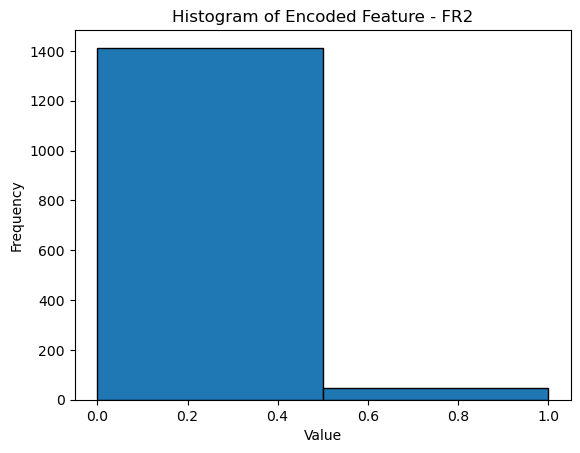
\includegraphics[width=.5\textwidth]{HW1/images/download3.png}\hfill
    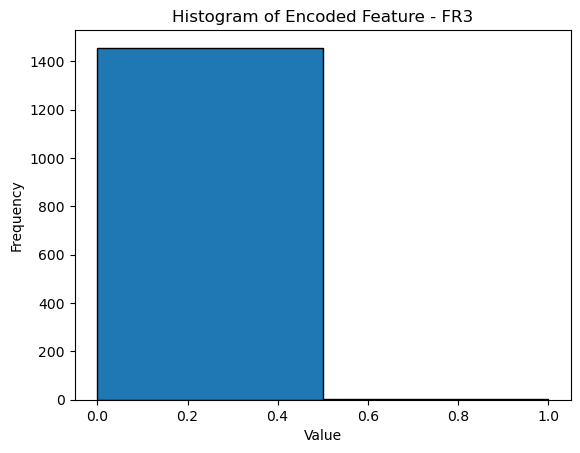
\includegraphics[width=.5\textwidth]{HW1/images/download4.png}\hfill
    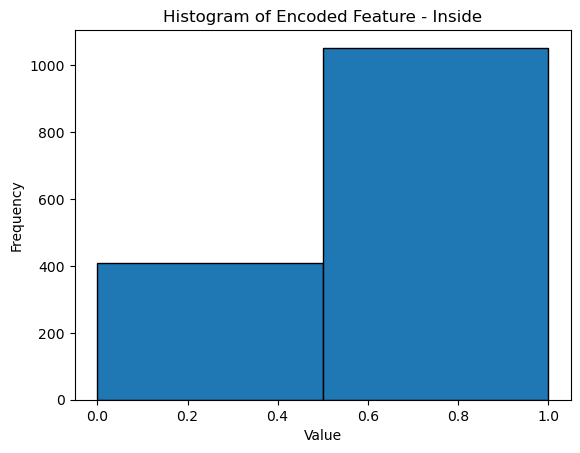
\includegraphics[width=.5\textwidth]{HW1/images/download5.png}
\end{figure*}

Now, we have 5 different subclasses that have transformed their data to reflect their categorical data numerically. 


The code for one-hot encoding is presented below

\begin{Solution}
\begin{lstlisting}[language=Python]
#performing encoding on all categorical features, and this is the only processing we will need
encoded_columns = pd.DataFrame()
encoded_columns = pd.get_dummies(categorical_features)   
# print(encoded_columns.head())
        
#concatenating the processed categorical and continuous data into 1 big pandas dataframe
finalData = pd.concat([encoded_columns, continuous_features], axis=1)
# print(finalData.info())
\end{lstlisting}
\end{Solution}

\begin{Problem}
    Using ordinary least squares (OLS), try to predict house prices on this dataset. Choose the features (or combinations of features) you would like to use or ignore, provided you justify your choice. Evaluate your predictions on the training set using the MSE and the $R^{2}$ score. For this question, you need to implement OLS from scratch without using any external libraries or packages.
\end{Problem}

\begin{Solution}

The features that we chose to drop are the initial columns that surpass the 33\% threshold of missing values. These are: ['Alley', 'FireplaceQu', 'PoolQC', 'Fence', 'MiscFeature']. Eventually, we also drop the 'Id' feature as well as the 'SalePrice' to prevent target leakage (and instead train it as a Y-Value in our model as displayed in the program below). This means that we are left with the remaining features shown below that would help us evaluate our training data sets.  

\begin{lstlisting}[language=Python]
['MSSubClass', 'MSZoning', 'LotFrontage', 'LotArea', 'Street', 'LotShape', 'LandContour', 'Utilities', 'LotConfig', 'LandSlope', 'Neighborhood', 'Condition1', 'Condition2', 'BldgType', 'HouseStyle', 'OverallQual', 'OverallCond', 'YearBuilt', 'YearRemodAdd', 'RoofStyle', 'RoofMatl', 'Exterior1st', 'Exterior2nd', 'MasVnrType', 'MasVnrArea', 'ExterQual', 'ExterCond', 'Foundation', 'BsmtQual', 'BsmtCond', 'BsmtExposure', 'BsmtFinType1', 'BsmtFinSF1', 'BsmtFinType2', 'BsmtFinSF2', 'BsmtUnfSF', 'TotalBsmtSF', 'Heating', 'HeatingQC', 'CentralAir', 'Electrical', '1stFlrSF', '2ndFlrSF', 'LowQualFinSF', 'GrLivArea', 'BsmtFullBath', 'BsmtHalfBath', 'FullBath', 'HalfBath', 'BedroomAbvGr', 'KitchenAbvGr', 'KitchenQual', 'TotRmsAbvGrd', 'Functional', 'Fireplaces', 'GarageType', 'GarageYrBlt', 'GarageFinish', 'GarageCars', 'GarageArea', 'GarageQual', 'GarageCond', 'PavedDrive', 'WoodDeckSF', 'OpenPorchSF', 'EnclosedPorch', '3SsnPorch', 'ScreenPorch', 'PoolArea', 'MiscVal', 'MoSold', 'YrSold', 'SaleType', 'SaleCondition']\end{lstlisting}


After running this code for our training data:
\begin{lstlisting}[language=Python]
import numpy as np
# Our parameters that minimize the mean squared objective for all of our columns
theta_best = np.linalg.solve(finalData.T.dot(finalData), finalData.T.dot(Y_train)) 
# print(theta_best)\end{lstlisting}

After processing our testing data (described in the below question) 
\begin{lstlisting}[language=Python]
from sklearn.metrics import r2_score
y_train_pred = finalData.dot(theta_best)
print(r2_score(Y_train, y_train_pred))\end{lstlisting}

resulted in a 0.9310337512792708 R-Score value, and a MSE score of 434955550.2062558, which makes some sense since we are dealing with houses that cost hundreds of thousands of dollars, and the difference is squared. These values are shown in our Jupyter Notebook. 

    
\end{Solution}

\begin{Problem}
    Train your model using all of the training data (all data points, but not necessarily all the features), and test it using the testing data. Submit your results to Kaggle.
\end{Problem}

\begin{Solution}

We processed our testing data the same way we processed our training data, and there are many overlaps in the feature engineering choices, so for the purposes of conciseness, we won't repeat the same explanations again. Here is what our pre-processing steps for our test data looks like: 

\begin{lstlisting}[language=Python]
# Read test data
X_test = pd.read_csv('house-prices-advanced-regression-techniques/test.csv')

# drop 
processing_testing_data = X_test
missing_percentage_test = (processing_testing_data.isnull().sum() / len(X_test)) * 100
columns_to_remove_test = missing_percentage_test[missing_percentage_test > 33].index.tolist()
# print(columns_to_remove)
cleaned_data_test = processing_testing_data.drop(columns=columns_to_remove_test)

continuous_features_test = cleaned_data_test.select_dtypes(include=[np.number])
categorical_features_test = cleaned_data_test.select_dtypes(exclude=[np.number])

# fill na with mean values
mean_values_test = continuous_features_test.mean()
continuous_features_test.fillna(mean_values_test, inplace=True)

# one-hot encoding
encoded_columns_test = pd.DataFrame()
encoded_columns_test = pd.get_dummies(categorical_features_test)  

# remove Id
finalData_test = pd.concat([encoded_columns_test, continuous_features_test], axis=1)
for col in finalData.columns: 
    if col not in finalData_test.columns: 
        finalData_test[col] = 0
        print(col)

finalData_test.drop('Id',axis=1,inplace = True)
finalData_test['one'] = 1
#Reordering our test columns with the training data set to avoid incompatible columns error
finalData_test = finalData_test[finalData.columns]

print(finalData_test.shape)
finalData_test.head()\end{lstlisting}

We submitted our solution to the Kaggle Competition, here's our results:

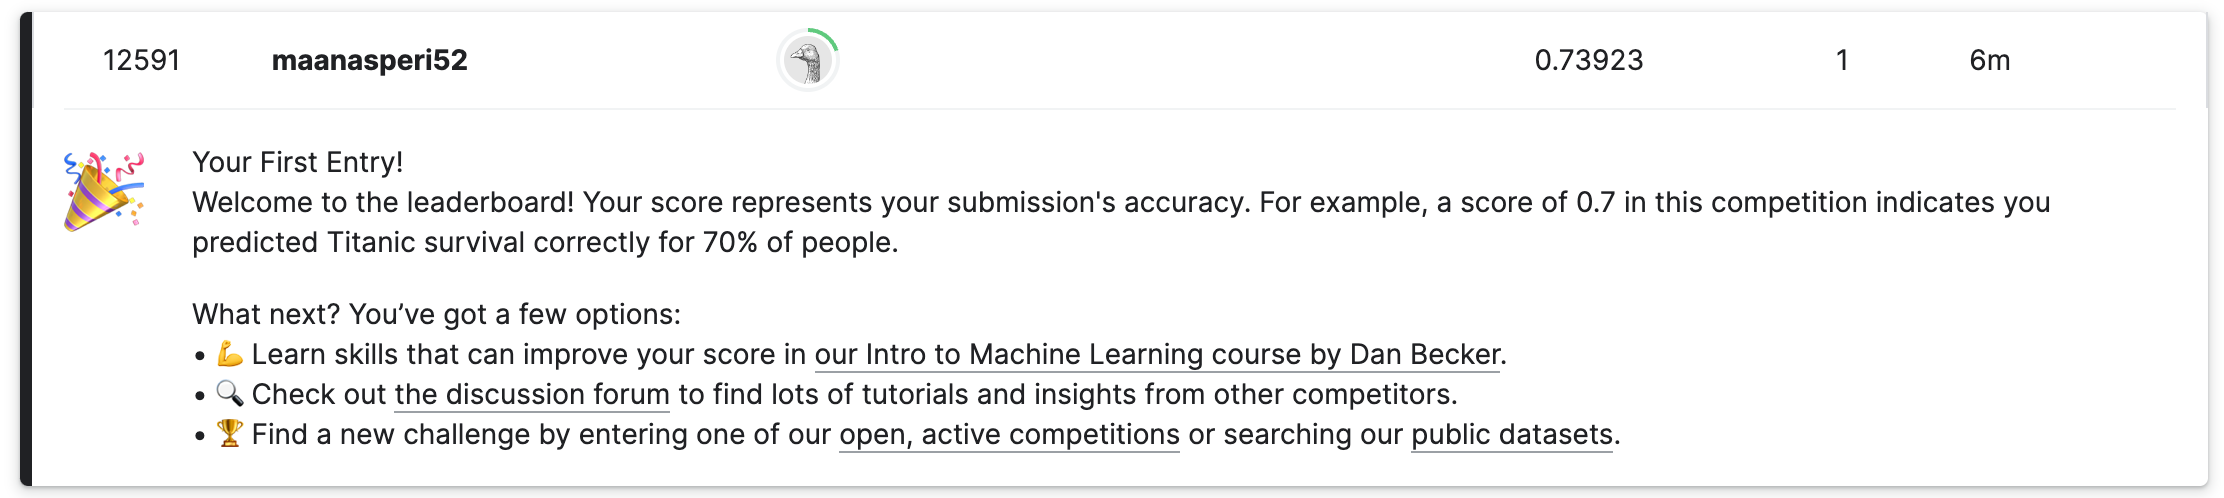
\includegraphics[max width=\textwidth, scale=1.0]{HW1/images/img10.png}


\end{Solution}

\section*{Part II: The Titanic Disaster}
\setcounter{Problem}{1}
\begin{Problem}
Implement logistic regression (it's ok to use sklearn or similar software packages), try to predict whether a passenger survived the disaster with your model. Choose the features (or combinations of features) you would like to use or ignore, provided you justify your choice.
\end{Problem}
\begin{Solution}
    The features we chose to ignore were:
    \begin{itemize}
        \item Name (technically, we included it just didn't encode this discrete variable)
        \item Cabin
        \item Ticket
    \end{itemize}
    The reasoning for dropping these features was because they do not really provide any useful information on the probability of survival of the passenger
\end{Solution}

\begin{Problem}
Train your classifier using all of the training data, and test it using the testing data. Submit your results to Kaggle.
\end{Problem}
\begin{Solution}

This is after our processing data, which is explained in detail in our jupyter notebook. We used the RandomForestClassifier because we wanted our model to replicate the unpredictable nature of a dense forest/data, where each tree in the forest represents a unique decision-making process. This may lead to overfitting, however, and in the future, we aim to allocate a bigger portion of the dataset for evaluation methods. 

\begin{lstlisting}[language=Python]
from sklearn.ensemble import RandomForestClassifier

#Now we can finally train and fit the model to our dataset
x_train = training.iloc[:,1:]
y_train = training.iloc[:,0:1]
x_test = testing.iloc[:,:]

model = RandomForestClassifier(n_estimators = 70)

x_train.columns = x_train.columns.astype(str)
y_train.columns = y_train.columns.astype(str)
x_test.columns = x_test.columns.astype(str)

model.fit(x_train,y_train)
y_pred= model.predict(x_test)
accuracy = model.score(x_train, y_train)

print(accuracy)
\end{lstlisting}

0.9820022497187851 was our scoring accuracy, as in 98.2\%, and after submitting to the Kaggle Competition, this was our leadership rankings. 

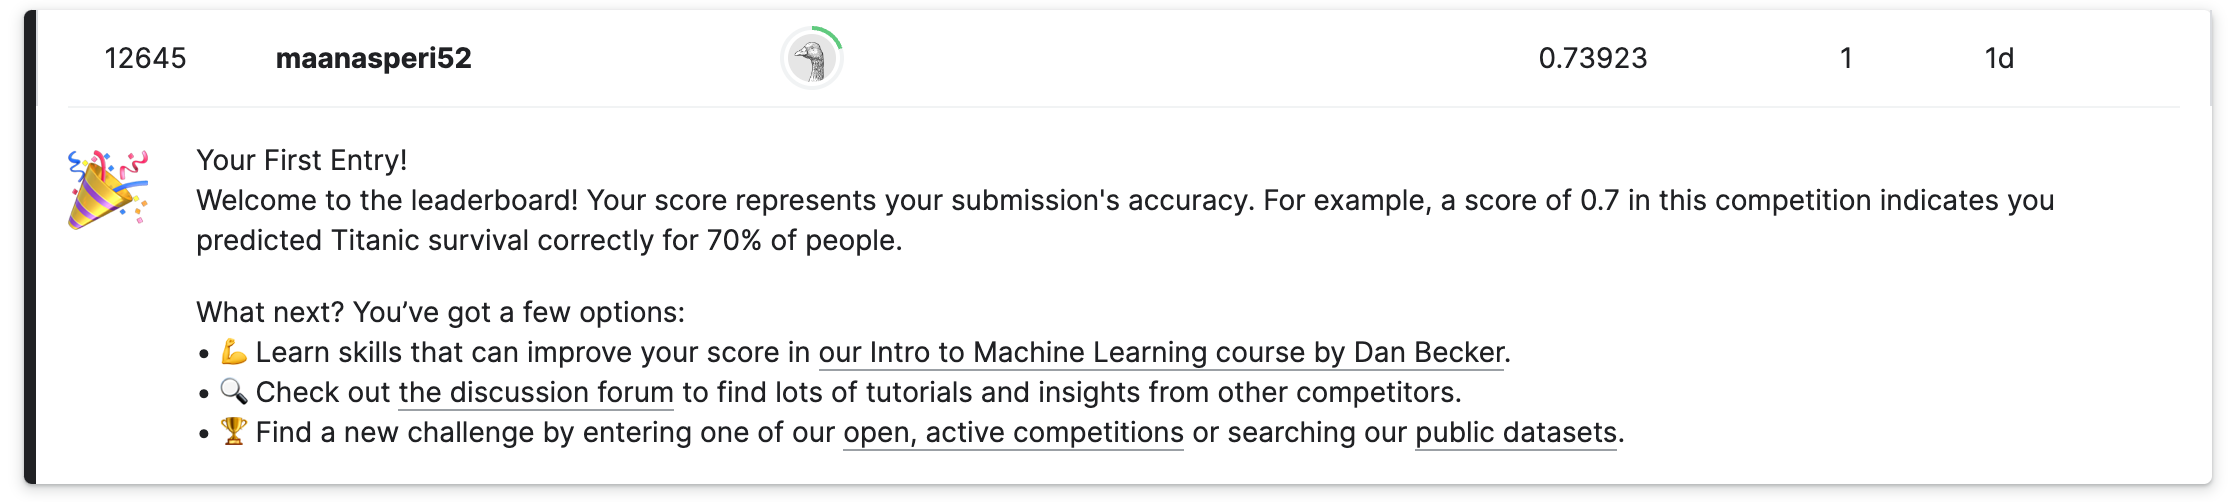
\includegraphics[max width=\textwidth, scale=1.0]{HW1/images/img11.png}


\end{Solution}

\section*{Written Exercises}

\setcounter{section}{0}

\section{Conceptual questions}

\begin{Problem*}[(a)]
Identify one advantage and one disadvantage of using gradient descent as the optimizer of a supervised linear model, compared to using the analytical formula based on the normal equations (as is done in the Ordinary Least Squares algorithm)
\end{Problem*}
\begin{Solution}

\textbf{Advantage:}\par
It’s great from an educational point of view because it teaches the concept of machine learning at a mathematical level that is understandable, and a concept that translates well to neural networks.\par
It’s excellent for large datasets, because you can partition data into chunks, and it can manage the computational demands of large data more effectively than other optimizing algorithms. This does not mean that it’s fast though, as discussed below in the disadvantages section. \\

\textbf{Disadvantage:}\par
Iteratively approaching the minimum takes a lot of time. Even with alternative methods of gradient descent and parallel computing, it’s a relatively slow algorithm to keep getting closer and closer to the desired minimum loss. \par
Gradient descent still does not arrive at the exact minimum value, even through multiple iterations. This is because arriving at the exact minimum is only as precise as the learning rate alpha. 
\end{Solution}

\begin{Problem*}[(b)]
Imagine doing a regression problem. You discretize the output space of $y$ into a large number of small intervals and apply a multi-class classification algorithm (like softmax regression) to predict the interval containing the target output. Would this approach be sufficient to solve the regression problem? Describe why or why not.\end{Problem*}
\begin{Solution}

Discretization is also known as the process of binning (dividing the range of the continuous variables into intervals), and this is a common method to train data. As long as the the thresholds of identifying the interval boundaries are accurate, this approach would be sufficient to solve the regression problem. Otherwise, poorly chosen intervals can make this algorithm make poor predictive choices when classifying data. \par
Using a multi-class classification algorithm, like softmax regression, is also optimal because regression algorithms are able to train faster and better using discrete values. Without these discrete values, the algorithms would have to exhaustively go through all the features for one value, whereas binning features would expedite the process.
\end{Solution}

\begin{Problem*}[(c)]
Name one advantage and one disadvantage of performing multi-class classification by training multiple one-vs-all classifiers compared to directly using a multi-class algorithm like softmax regression.\end{Problem*}
\begin{Solution}

\textbf{Advantage:}\par
Training a one-vs-all algorithm prepares a binary classifier for every single K classification type. These classifiers are trained separately for each different type of outcome, and the collection of these classifiers results in a multi-classification solution. This makes interpreting the values simple because of the simplified nature of binary classifiers, and easy to determine which classifier is providing more inaccurate results than the other. Furthermore, each of these classifiers is compatible with a number of models, such as linear models, decision trees, logistic regression, etc. Last but not least, each binary classifier can have its own parameters, allowing for more control over each and every classifier. \par

\textbf{Disadvantage:}\par
The biggest disadvantage of a one-vs-all classifier is the class imbalance that occurs. For example, if there is a 90-10\% distribution of Dataset A to Dataset B, then there won’t be enough conclusive data to understand the prediction patterns of Dataset B. Classifiers are prone to struggle against skewed data. Even in the case of a 5-class classification problem, if there are 5 classes with a roughly equal 20\% dataset distribution, each of these 5 classes ends up with a 20-80\% distribution (class vs rest of classes). 
\end{Solution}

\begin{Problem*}[(d)]
The computational complexity of polynomial regression depends on the number of data points in the training set and on the degree of the polynomial that we are trying to fit.

\begin{enumerate}
    \item[\textbf{(i.)}] Assuming that each data point has $d$ attributes and we want our model class to consist of all polynomials of $d$ variables and degree at most $p$, state the dimension of the polynomial features that are needed to implement this model class. Specifying a big-Oh estimate is enough.

    \item[\textbf{(ii.)}] State the computational complexity of applying polynomial least squares with the above set of polynomial features. Again, a big-Oh estimate is sufficient.

    \item[\textbf{(iii.)}] Comment on how the above findings may influence your decision for when to apply polynomial regression in real-world settings.

\end{enumerate}

\end{Problem*}
\begin{Solution}
\begin{enumerate}

\item[\textbf{(i.)}] $O(p^d)$

\item[\textbf{(ii.)}] $O(n*p^d)$

\item[\textbf{(iii.)}] It is prohibitively expensive to use high-degree polynomial regression given a large dataset with large number of attributes, there needs to be a trade-off
\end{enumerate}
\end{Solution}

\section{Analytical solution for Ordinary Least Squares}

\begin{Problem*}
Analytical solution for Ordinary Least Squares. Consider a simple dataset of $n$ training instances $\left\{\left(x^{(1)}, y^{(1)}\right),\left(x^{(2)}, y^{(2)}\right), \ldots,\left(x^{(n)}, y^{(n)}\right)\right\}$, with inputs $x^{(i)} \in \mathbb{R}$ and targets $y^{(i)} \in \mathbb{R}$. We are going to fit a simple linear model with parameters $\theta=\left(\theta_{0}, \theta_{1}\right)$ on this dataset:

$$
f_{\theta}(x)=\theta_{0}+\theta_{1} x^{(i)} .
$$

We define the learning objective to be the residual sum of squares, parameterized by $\theta_{0}, \theta_{1}$ :

$$
J\left(\theta_{0}, \theta_{1}\right)=\sum_{i=1}^{n}\left(y^{(i)}-f_{\theta}(x)^{(i)}\right)^{2}
$$

Instead of using gradient descent, which works in an iterative manner, we will derive a formula for the parameters that minimize the objective $J$.
\end{Problem*} 

\begin{Problem*}[(a)]
    Calculate the partial derivatives $\frac{\partial}{\partial \theta_{0}} J\left(\theta_{0}, \theta_{1}\right)$ and $\frac{\partial}{\partial \theta_{1}} J\left(\theta_{0}, \theta_{1}\right)$.
\end{Problem*}

\begin{Solution}
    \begin{align}
    \begin{split}
        \frac{\partial}{\partial \theta_{0}} J\left(\theta_{0}, \theta_{1}\right) &= \frac{\partial}{\partial \theta_{0}} \sum_{i=1}^{n}\left(y^{(i)}-f_{\theta}(x)^{(i)}\right)^{2} \\
        &= \frac{\partial}{\partial \theta_{0}} \sum_{i=1}^{n}\left(y^{(i)}-\theta_{0}-\theta_{1} x^{(i)}\right)^{2} \\
        &= \sum_{i=1}^{n} -2*\left(y^{(i)}-\theta_{0}-\theta_{1} x^{(i)}\right) \\
        &= \boxed{2\sum_{i=1}^{n} \left(\theta_{0} + \theta_{1} x^{(i)} - y^{(i)}\right)}
    \end{split}
  \end{align}

    \begin{align}
    \begin{split}
        \frac{\partial}{\partial \theta_{1}} J\left(\theta_{0}, \theta_{1}\right) &= \frac{\partial}{\partial \theta_{1}} \sum_{i=1}^{n}\left(y^{(i)}-f_{\theta}(x)^{(i)}\right)^{2} \\
        &= \frac{\partial}{\partial \theta_{1}} \sum_{i=1}^{n}\left(y^{(i)}-\theta_{0}-\theta_{1} x^{(i)}\right)^{2} \\
        &= \sum_{i=1}^{n} -2x^{(i)}*\left(y^{(i)}-\theta_{0}-\theta_{1} x^{(i)}\right) \\
        &= \boxed{2\sum_{i=1}^{n} x^{(i)}\left(\theta_{0} + \theta_{1} x^{(i)} - y^{(i)}\right)}
    \end{split}
  \end{align}
\end{Solution}

\begin{Problem*}[(b)]
    Consider the fact that $J\left(\theta_{0}, \theta_{1}\right)$ has an unique optimum ${ }^{1}$, which we denote as $\theta_{0}^{*}, \theta_{1}^{*}$. We can obtain the analytical solution for $\theta_{0}^{*}, \theta_{1}^{*}$ by setting the gradient of $J$ to zero, which yields the following normal equations:

\footnotetext{${ }^{1} J\left(\theta_{0}, \theta_{1}\right)$, the cost function for linear regression, has a unique optimum (i.e., a global minimum). The technical reason for this fact is that $J$ is a convex function, which can be verified, for example, by showing that its Hessian is positive semidefinite.}

$$
\begin{aligned}
& \frac{\partial}{\partial \theta_{0}} J\left(\theta_{0}^{*}, \theta_{1}\right)=0 \\
& \frac{\partial}{\partial \theta_{1}} J\left(\theta_{0}, \theta_{1}^{*}\right)=0
\end{aligned}
$$

Write out the above equations and use them to prove the following properties:

$$
\theta_{0}^{*}=\bar{y}-\theta_{1} \bar{x}
$$

and

$$
\theta_{1}^{*}=\frac{\sum_{i=1}^{n} x^{(i)}\left(y^{(i)}-\bar{y}\right)}{\sum_{i=1}^{n} x^{(i)}\left(x^{(i)}-\bar{x}\right)}
$$

(Note: $\bar{x}=\frac{1}{n} \sum_{i=1}^{n} x^{(i)}$ and $\bar{y}=\frac{1}{n} \sum_{i=1}^{n} y^{(i)}$.)
\end{Problem*}

\begin{Solution}

     $$\frac{\partial}{\partial \theta_{0}} J\left(\theta_{0}^{*}, \theta_{1}\right) = 2 * \sum_{i=1}^{n} \left(\theta_{0}^{*} + \theta_{1} x^{(i)} - y^{(i)}\right) = 0 $$
    
    $$\sum_{i=1}^{n}\theta_{0}^{*} + \sum_{i=1}^{n}\theta_{1} x^{(i)} - \sum_{i=1}^{n}y^{(i)} = 0$$
    
    $$\sum_{i=1}^{n}\theta_{0}^{*} = \sum_{i=1}^{n}y^{(i)} - \sum_{i=1}^{n}\theta_{1} x^{(i)}$$

    $$\theta_{0}^{*} * n = \sum_{i=1}^{n}y^{(i)} - \sum_{i=1}^{n}\theta_{1} x^{(i)}$$

    $$\theta_{0}^{*} = \frac{1}{n}\sum_{i=1}^{n}y^{(i)} - \frac{1}{n}\sum_{i=1}^{n}\theta_{1} x^{(i)}$$

    \begin{equation}
    \boxed{
    \begin{array}{rcl}
    \theta_{0}^{*} = \bar{y}-\theta_{1} \bar{x}
    \end{array}
    }
    \end{equation}

     $$\frac{\partial}{\partial \theta_{1}} J\left(\theta_{0}, \theta_{1}^{*}\right) = 2 * \sum_{i=1}^{n} x^{(i)}*\left(\theta_{0} + \theta_{1}^{*} x^{(i)} - y^{(i)}\right) = 0 $$
    
    $$ \sum_{i=1}^{n} x^{(i)}*\left(\bar{y}-\theta_{1} \bar{x} + \theta_{1}^{*} x^{(i)} - y^{(i)}\right) = 0 $$

    $$ \sum_{i=1}^{n} \bar{y}x^{(i)} - \theta_{1} \bar{x} x^{(i)} + \theta_{1}^{*} x^{2(i)} - y^{(i)}x^{(i)} = 0 $$

    $$ \sum_{i=1}^{n} \theta_{1}^{*} x^{2(i)} - \theta_{1} \bar{x} x^{(i)} = \sum_{i=1}^{n} y^{(i)}x^{(i)} - \bar{y}x^{(i)}  $$

    $$ \theta_{1} \sum_{i=1}^{n} x^{(i)}\left(x^{(i)} - \bar{x}\right) = \sum_{i=1}^{n} x^{(i)}\left(y^{(i)} - \bar{y}\right)  $$
    
    \begin{equation}
    \boxed{
    \begin{array}{rcl}
    \theta_{1}^{*}=\frac{\sum_{i=1}^{n} x^{(i)}\left(y^{(i)}-\bar{y}\right)}{\sum_{i=1}^{n} x^{(i)}\left(x^{(i)}-\bar{x}\right)}
    \end{array}
    }
    \end{equation}

\end{Solution}

\begin{Problem*}[(c)]
For the optimal $\theta_{0}^{*}, \theta_{1}^{*}$, calculate the sum of the residuals $$\sum_{i=1}^{n} e^{(i)}=\sum_{i=1}^{n}\left(y^{(i)}-\left(\theta_{0}^{*}+\theta_{1}^{*} x^{(i)}\right)\right)$$. What can you learn from the value of $\sum_{i=1}^{n} e^{(i)}$?
\end{Problem*}

\begin{Solution}
    \begin{align}
    \begin{split}
        \sum_{i=1}^{n}e^{(i)} &= \sum_{i=1}^{n}\left(y^{(i)}-\left(\theta_{0}^{*}+\theta_{1}^{*} x^{(i)}\right)\right) \\
        &= \sum_{i=1}^{n}\left(y^{(i)} - \bar{y} + \theta_{1}\bar{x} - \theta_{1}^{*} x^{(i)}\right) \\
        &= \sum_{i=1}^{n}\left(y^{(i)} - \bar{y} + \theta_{1}\left(\bar{x} - x^{(i)}\right)\right) \\
        &= \sum_{i=1}^{n}\left(y^{(i)} - \bar{y} + \frac{x^{(i)}\left(y^{(i)}-\bar{y}\right)}{x^{(i)}\left(x^{(i)}-\bar{x}\right)} \left(\bar{x} - x^{(i)}\right)\right) \\
        &= \sum_{i=1}^{n}\left(y^{(i)} - \bar{y} + \frac{\cancel{x^{(i)}}\left(y^{(i)}-\bar{y}\right)}{\cancel{x^{(i)}} \cancel{\left(x^{(i)}-\bar{x}\right)}} \cancel{\left(x^{(i)}-\bar{x}\right)}\right) \\
        &= \sum_{i=1}^{n}\left(2y^{(i)} - 2\bar{y} \right)\\
        &= 2\sum_{i=1}^{n}\left(y^{(i)}\right) - 2\bar{y}\sum_{i=1}^{n}\left(1 \right)\\
        &= 2n\bar{y} - 2\bar{y}n\\
        &= \boxed{0}
    \end{split}
    \end{align}
Sum of residuals for linear regression model is zero, which means that the line runs perfectly in the middle of data points. So positive residuals cancel out negative residuals, thus the sum is 0.
\end{Solution}

\section{Maximum Likelihood Estimation}

\begin{Problem*}[(a)]
You are conducting an experiment involving the tossing of a four-sided dice. You conducted eight dice throws and meticulously recorded the outcomes. Your objective is to determine from this dataset the true probabilities of the dice falling on each of its four sides (which we denote by $1,2,3,4)$.

The dataset $D=\{3,2,3,4,4,4,2,4\}$, shown in Table 1, consists of the recorded outcomes of the eight dice throws. Each $x^{(i)} \in D$ refers to an individual throw. Each throw in Table 1 is represented by a throw number and a corresponding outcome (e.g., the dice landed on value '3' in throw number 1).

\begin{center}
\begin{tabular}{|c|c|}
\hline
Throw Number & Outcome \\
\hline
1 & 3 \\
2 & 2 \\
3 & 3 \\
4 & 4 \\
5 & 4 \\
6 & 4 \\
7 & 2 \\
8 & 4 \\
\hline
\end{tabular}
\end{center}

Table 1: Results of Eight Sample Throws of the 4-sided Dice

\end{Problem*}

\begin{Problem*}[i. Probabilistic Model. ]
Construct a probabilistic model that captures the underlying probabilities governing the dice outcomes. Define the model and its parameters, aiming to establish the probabilities associated with each outcome.
\end{Problem*}

\begin{Solution}
\begin{itemize}
    \item There are four possible outcomes: 1, 2, 3, 4. A training dataset consists dice throws,  $D=\{3,2,3,4,4,4,2,4\}$

    \item Our task is to estimate the true probability of each dice throw

    \item That being said, it means that we will have 4 parameters
    \begin{itemizedot}
        \item $P_\theta(x = j): \theta_j$ where $\theta_j \in [0,1]$
    \end{itemizedot}
    

    
\end{itemize}
    

    
\end{Solution}

\begin{Problem*}[ii. Learning Paradigm. ]
Classify the experiment as fitting into supervised learning, unsupervised learning, or reinforcement learning paradigms.
\end{Problem*}

\begin{Solution}
    The experiment fits into supervised learning paradigm
\end{Solution}

\begin{Problem*}[(b)]
Write a formula for the log-likelihood of the dataset under the probabilistic model. Provide an intuitive argument for why we would want to optimize this objective.
\end{Problem*}

\begin{Solution}


\begin{align}
    \begin{split}
        L(\theta) &= \prod_{i=1}^n P_\theta(x^{(i)}) \\ 
        &=\theta_3 \cdot \theta_2 \cdot \theta_3 \cdot \theta_4 \cdot \theta_4 \cdot \theta_4 \cdot \theta_2 \cdot \theta_4\\
        & =\theta^{\# \text { 1's }} \cdot \theta^{\# \text { 2's }} \cdot \theta^{\# \text { 3's }} \cdot \theta^{\# \text { 4's }}\\
        \log L(\theta) & =\log \left(\theta_1^{\# \text { 1's }} \cdot \theta_2^{\# \text { 2's }} \cdot \theta_3^{\# \text { 3's }} \cdot \theta_4^{\# \text { 4's }} \right)\\
        & =\# \text { 1's } \cdot \log (\theta_1)+\# \text { 2's } \cdot \log (\theta_2) +\# \text { 3's } \cdot \log (\theta_3) +\# \text { 4's } \cdot \log (\theta_4)\\
        &= 2 \cdot \log (\theta_2) + 2 \cdot \log (\theta_3) + 4 \cdot \log (\theta_4)
    \end{split}
\end{align}

We want to optimize the probabilities of the observed dataset.

\end{Solution}

\begin{Problem*}[(c)]
Calculate the maximum likelihood estimate of the model parameters. Interpret the parameter values within the context of dice toss probabilities, considering how they relate to the observed outcomes.
\end{Problem*}

\begin{Solution}
    \begin{align}
    \begin{split}
        \frac{\partial \log L(\theta)}{\partial \theta_1} &= 0 \\
        \\
        \frac{\partial \log L(\theta)}{\partial \theta_2} &= \frac{2}{\theta_2} \\
        \\
        \frac{\partial \log L(\theta)}{\partial \theta_3} &= \frac{2}{\theta_3} \\
        \\
        \frac{\partial \log L(\theta)}{\partial \theta_4} &= \frac{4}{\theta_4} \\
        \\
        \frac{2}{\theta_2} = \frac{2}{\theta_3} = \frac{4}{\theta_4} , \text{where} \sum_{i=1}^{4} = 1 \\
        \\ 
        \boxed{\theta_1 = 0, \theta_2 = 0.25, \theta_3 = 0.25, \theta_4 = 0.5}
    \end{split}
\end{align}
\end{Solution}

\begin{Problem*}[(d.)]
Recognize scenarios where this approach might yield inaccurate estimates of the true probabilities of the dice falling on each of its four sides. Provide at least one example and elucidate the reasoning behind potential inaccuracies.
\end{Problem*}

\begin{Solution}
    Small data sets. Theoretically it makes sense if a 4 sided die will have an equal probability to land on each of its sides. However, given the dataset, this approach suggests other probabilities, akin to a loaded die. Increasing the dataset will remove these inaccuracies.
\end{Solution}


%%%%%%%%%%%%%%%%%%%%%%%%%%%%%%%%%%%%%%%%%%%%%%%%%%%%%%%%%%%%%%%%%%
%Complete the assignment now
\end{document}

%%%%%%%%%%%%%%%%%%%%%%%%%%%%%%%%%%%%%%%%%%%%%%%%%%%%%%%%%%%%%%%%%%
%%%%%%%%%%%%%%%%%%%%%%%%%%%%%%%%%%%%%%%%%%%%%%%%%%%%%%%%%%%%%%%%%%
